\documentclass[11pt, a4paper, twoside]{article}

% Version en 2024 Víctor Bettachini < vbettachini@unlam.edu.ar >

\usepackage[T1]{fontenc}
\usepackage[utf8]{inputenc}

% \usepackage[spanish, es-tabla]{babel}
% \def\spanishoptions{argentina} % Was macht dass?
% \usepackage{babelbib}
% \selectbiblanguage{spanish}
% \addto\shorthandsspanish{\spanishdeactivate{~<>}}

\usepackage{graphicx}
\graphicspath{{../figuresLaTeX/}}
% \usepackage{float}

\usepackage[arrowdel]{physics}
\newcommand{\pvec}[1]{\vec{#1}\mkern2mu\vphantom{#1}}
% \usepackage{units}
\usepackage[separate-uncertainty= true, multi-part-units= single, range-units= single, range-phrase= {~a~}, locale= FR]{siunitx}
\usepackage{isotope} % $\isotope[A][Z]{X}\to\isotope[A-4][Z-2]{Y}+\isotope[4][2]{\alpha}

\usepackage{tasks}
\usepackage[inline]{enumitem}
% \usepackage{enumerate}

\usepackage{hyperref}

% \usepackage{amsmath}
% \usepackage{amstext}
% \usepackage{amssymb}

\usepackage{tikz}
\usepackage{tikz-3dplot}
\usepackage{tikz-dimline}
\usetikzlibrary{calc}
% \usetikzlibrary{math}
\usetikzlibrary{arrows.meta}
\usetikzlibrary{snakes}
\usetikzlibrary{decorations}
\usetikzlibrary{decorations.pathmorphing}
\usetikzlibrary{patterns}

\usepackage[hmargin=1cm,vmargin=3cm, top= 0.75cm,nohead]{geometry}

\usepackage{lastpage}
\usepackage{fancyhdr}
\pagestyle{fancyplain}
\fancyhf{}
\setlength\headheight{28.7pt} 
\fancyhead[LE, LO]{\textbf{Computational Analytical Mechanics} }
% \fancyhead[LE, LO]{\textbf{Mecánica General} }
\fancyhead[RE, RO]{\href{https://ingenieria.unlam.edu.ar/}{$\vcenter{\hbox{\includegraphics[height=1cm]{ambos.pdf}}}$}}
\fancyfoot{\href{https://creativecommons.org/licenses/by-nc-sa/4.0/}{$\vcenter{\hbox{\includegraphics[height=0.4cm]{by-nc-sa_80x15.pdf}}}$} \href{https://ingenieria.unlam.edu.ar/}{DIIT - UNLaM}}
\fancyfoot[C]{ {\tiny Updated \today} }
\fancyfoot[RO, LE]{Page \thepage/\pageref{LastPage}}
\renewcommand{\headrulewidth}{0pt}
\renewcommand{\footrulewidth}{0pt}


\begin{document}
\begin{center}
  \textsc{\large External forces in the Lagrangian formulation}
\end{center}

\begin{enumerate}

\item 
%\textbf{MIT Pset ? ex ?} 
\begin{minipage}[t][4.8cm]{0.55\textwidth} 
\textbf{Rod hanging from a cart}\\
Find the dynamics equations for the system.
The moment of inertia for a rod of mass \(m\) and length \(l\) about an axis passing through one end of the rod is \(\frac{m}{12} l^2\). 
\begin{enumerate}
	\item Write the Lagrangian.
	\item Write the nonconservative forces as generalized forces:
	\begin{itemize}
		\item the external force \(\vec{F}(t)\),
		\item and the force exerted by the dumping system of constant \(b\) as a function of the cart's velocity, \(- b \dot{x} \hat{x}\).
	\end{itemize}
	\item Find the Euler-Lagrange equations. 
\end{enumerate}
\end{minipage}
\begin{minipage}[c][0cm][t]{0.4\textwidth}
	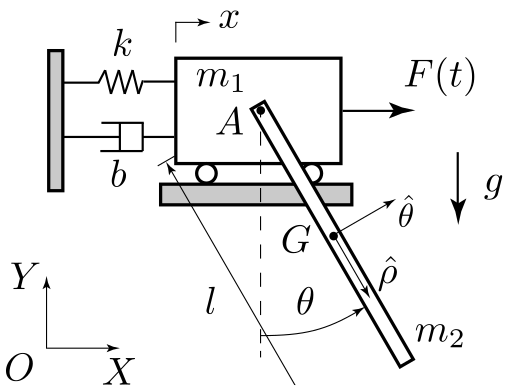
\includegraphics[width=\textwidth]{figures/zweite}
\end{minipage}




\item 
%\textbf{MIT Pset 7 ex 2} 
\begin{minipage}[t][5.5cm]{0.6\textwidth}
\textbf{Unbalanced torsion pendulum}\\
Two beads of identical masses $m$ are attached to the ends of arms of negligible mass.
One of these arms is inclined at a fixed angle $\phi$ with respect to the horizontal.
There is no friction with the system that keeps the axis of rotation vertical.
This axis is free to rotate at any angle $\theta$ and a torsion spring of constant $K_t$ exerts an opposite torque each time $\theta \neq 0$.
Additionally to this torque, there is an external torque that is a function of time: $\vec{\tau}= \tau (t) \hat{z}$.

Question:
What is the unit for the generalized force?
\begin{tasks}(5)
	\task \si{\newton}
	\task \si{\newton \over \metre}
	\task \si{\newton \metre}
	\task Other
\end{tasks}
Solve for the angular acceleration using the Euler-Lagrange equation for the dynamics of this system. Result:
\[
	\ddot{\theta} = \frac{K_{T} \theta + \tau}{L^{2} m \left(\sin^{2}{\left(\phi \right)} - 2\right)}
\] 
\end{minipage}
\begin{minipage}[c][1cm][t]{0.35\textwidth}
	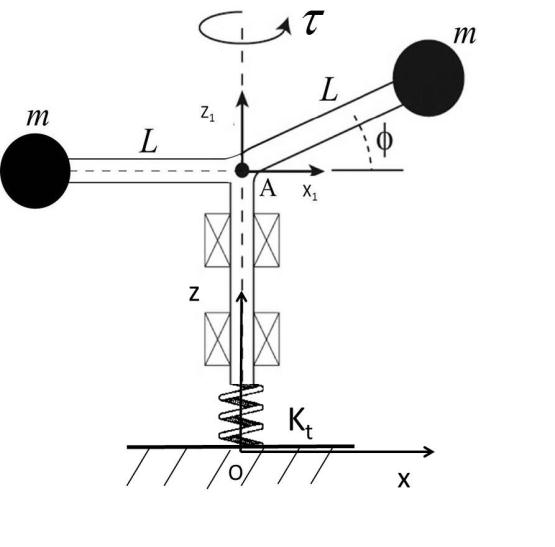
\includegraphics[width=\textwidth]{figures/pset7ex2}
\end{minipage}



\item
%\textbf{MIT Pset 7 ex 4} 
\begin{minipage}[t][8cm]{0.6\textwidth}
\textbf{Fixed cylinders}\\
Two homogeneous cylinders of masses and radii $m_1$,$m_2$, $R_1$ and $R_2$ are welded together.
This arrangement rotates without friction about an axis.
A string of negligible mass is wounded around the external cylinder and its ends connect a spring of constant $k$ and a damper.
This damper exerts a force opposite to the linear velocity,
$$
\vec{F}_\mathrm{damper} = - b \dot{\vec{r}}.
$$
A string of negligible mass is wrapped around the cylinder with the smaller radius, and a block of mass $m_o$ hangs from it.\\
Solve for the angular acceleration using the Euler-Lagrange equation. 
Result:\\
\[
	\ddot{\theta} = \frac{2 \left(R_{1} g m_{0} - R_{2}^{2} b \dot{\theta} - R_{2}^{2} k \theta\right)}{2 R_{1}^{2} m_{0} + R_{1}^{2} m_{1} + R_{2}^{2} m_{2}}
\]
\end{minipage}
\begin{minipage}[c][0cm][t]{0.35\textwidth}
	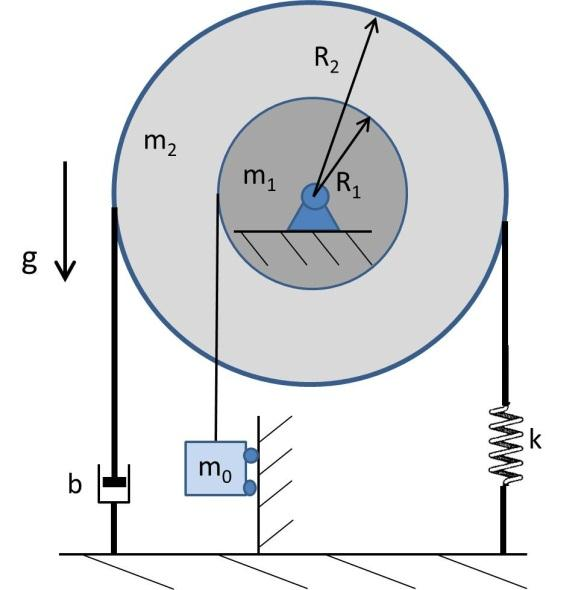
\includegraphics[width=\textwidth]{figures/pset7ex4}
\end{minipage}



\item
%\textbf{MIT Pset 7 ex 6} 
\begin{minipage}[t][6cm]{0.5\textwidth}
\textbf{Oscillating inclined plane}\\
A disk of radius $R$ and mass $m$ rotates over the surface of the cart of mass $m_0$, inclined at an angle $\theta_0$.
This disk won't leave the surface, even when the force $\vec{F}= F(t) \hat{x}$ is exerted upon it, due to a spring of constant $K_1$ that links its center with the cart.
There is also a spring of constant $K_2$ attached to the wall and a damper, proportional to the velocity, of constant $b$.
Both springs are initially at their natural lengths $l_{10}$ and $l_{20}$.
There is no friction between the cart and the floor.\\
\end{minipage}
\begin{minipage}[c][0cm][t]{0.45\textwidth}
	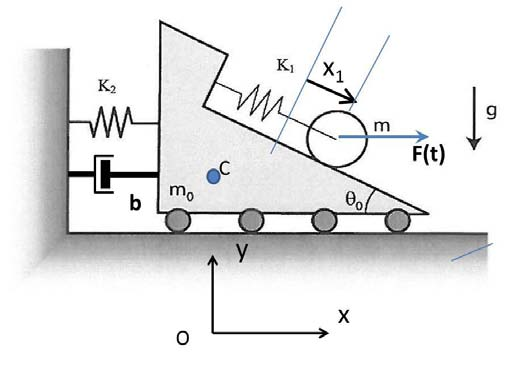
\includegraphics[width=\textwidth]{figures/pset7ex6}
\end{minipage}
Question: What is the expression for the generalized force corresponding to the virtual displacement $\delta x$ due to $\vec{F}$?\\
\begin{tasks}(4)
	\task $F(t) \cos(\theta)$
	\task $F(t)$
	\task $F(t) \delta x$
	\task $0$
\end{tasks}
Find the Euler-Lagrange equations. 



\end{enumerate}
\end{document}
